\paragraph{L'interface DAO}

\begin{minipage}
    {\linewidth}
    \centering
    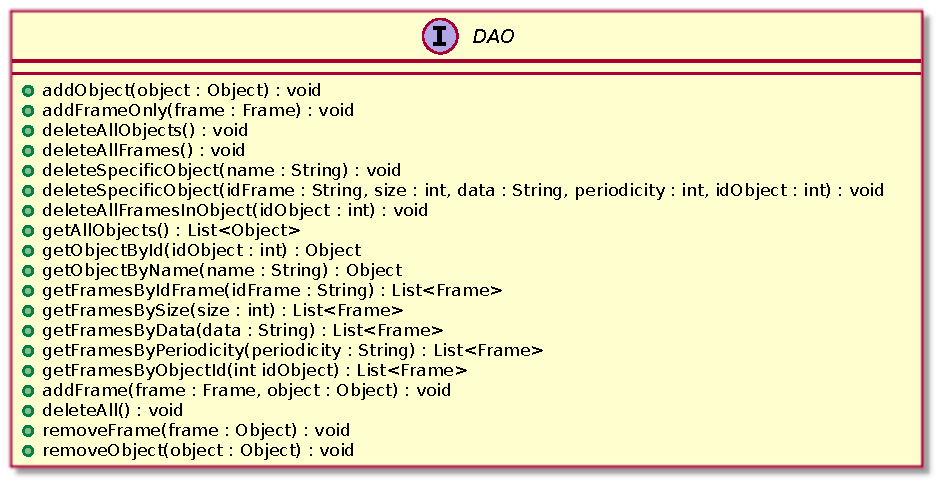
\includegraphics[width=0.80\linewidth]{../schemas/Conception_detaillee/interface_dao.pdf}
    \captionof{figure}{Diagramme de l'interface DAO}
\end{minipage}

\subparagraph{Philosophie de conception \newline} 

\medspace

L'interface DAO définit les différents accès possibles à la base de données.

\subparagraph{Description structurelle \newline}

\medspace

\textbf{Attributs :}

N.A. 


\textbf{Services offerts :}

\begin{itemize}
    \item \textbf{addObject(object : Object) : void } --- Opération qui permet d'ajouter un objet à la base de données.
    \item \textbf{addFrameOnly(frame : Frame) : void } --- Opération qui permet d'ajouter une trame à la base de données.
    \item \textbf{deleteAllObjects() : void } --- Opération qui permet de supprimer tous les objets de la base de données. 
    \item \textbf{deleteAllFrames() : void } --- Opération qui permet de supprimer toutes les trames de la base de données.
    \item \textbf{deleteSpecificObject(name : String) : void } --- Opération qui permet de supprimer un objet précis dans la base de données.
    \item \textbf{deleteSpecificFrame(idFrame : String, size : int, data : String, periodicity : int, idObject : int) : void } --- Opération qui permet de supprimer une trame précise dans la base de données. 
    \item \textbf{deleteAllFramesInObject(idObject : int) : void } --- Opération qui permet de supprimer toutes les trames dans un objet. 
    \item \textbf{getAllObjects() : List<Object> } --- Opération qui permet de sélectionner tous les objets créés. 
    \item \textbf{getObjectById(idObject : int) : Object } --- Opération qui permet de chercher un objet selon son identifiant. 
    \item \textbf{getObjectByName(name : String) : Object } --- Opération qui permet de chercher un objet selon son nom. 
    \item \textbf{getFramesByIdFrame(idFrame : String) : List<Frame> } --- Opération qui permet de chercher une ou plusieurs trames selon leur identifiant de trame.
    \item \textbf{getFramesBySize(size : int) : List<Frame> } --- Opération qui permet de chercher une ou plusieurs trames selon leur taille.
    \item \textbf{getFramesByData(data : String) : List<Frame> } --- Opération qui permet de chercher une ou plusieurs trames selon leur message.
    \item \textbf{getFramesByPeriodicity(periodicity : String) : List<Frame> } --- Opération qui permet de chercher une ou plusieurs trames selon leur périodicité.
    \item \textbf{getFramesByObjectId(int idObject) : List<Frame> } --- Opération qui permet de chercher une ou plusieurs trames selon leur identifant d'objet.
    \item \textbf{addFrame(frame : Frame, object : Object) : void } --- Opération qui permet d'ajouter une trame en fonction d'un objet. Cette opération appelle l'opération qui ajoute la trame à la base de données tout en la liant avec un objet. 
    \item \textbf{deleteAll() : void } --- Opération qui permet de supprimer tous les éléments de la base de données. 
    \item \textbf{removeFrame(frame : Object) : void } --- Opération qui permet de supprimer une trame précisement en ne fournissant en paramètre que la trame à supprimer au lieu des différents paramètres. 
    \item \textbf{removeObject(object : Object) : void } --- Opération qui permet de supprimer un objet précisement en ne fournissant en paramètre que l'objet à supprimer au lieu des différents paramètres.  
\end{itemize}

